\documentclass[a4paper]{article}

%% Language and font encodings
\usepackage[english]{babel}
\usepackage[utf8x]{inputenc}
\usepackage[T1]{fontenc}

%% Sets page size and margins
\usepackage[a4paper,top=3cm,bottom=2cm,left=2cm,right=2cm,marginparwidth=1.75cm]{geometry}

%% Useful packages
\usepackage{amsmath}
\usepackage{graphicx}
\usepackage[colorinlistoftodos]{todonotes}
\usepackage[colorlinks=true, allcolors=blue]{hyperref}

\title{Developing the Development Indices: A Data-Driven Approach to Scoring World Economies on Comprehensive Measures}
\author{Lingfeng Cheng, Mihir Paradkar, Yuting Tian}

\begin{document}
\maketitle



\section{Project Objective}
Scoring the development level of different nations is of vital importance to many entities, from corporations looking to make investments to governments formulating strategic plans. While there are various measures to quantify the development level, the clustering based method is among the most straightforward approaches. Through comparing with the countries in both the same and different clusters, investors, politicians and the public are able to form a basic perception of the nation. While many organizations like the World Bank, Fragile State Index provide certain clustering result, they are mostly economic based, with many other perspectives such as education, environment, and infrastructure underweighted. In contrast, our objective is to develop various clustering results based on a wide range of indicators such as health, economic, and environment, extracted from the World Bank's World Development Indicators (WDI) dataset. In this way, investors, politicians, and the public will form a comprehensive view of the nation's advantage and disadvantage. 
\section{Approach}
\subsection{Dataset Description}
The WDI dataset is collected by the World Bank and updated quarterly. The reason of using this dataset is because it presents the most up-to-date and accurate global development data and covers a wide range of perspectives such as agriculture, environment, education and infrastructure for every country and some aggregate regions in the world. Furthermore, for each perspective, a large number of indicators are proposed, with the corresponding data collected annually since 1960. We believe these historical data augment the amount of information available to fit a model and also can help predict categories better by accounting for changes in indicators for particular regions. The numbers for each indicator are real-valued (no nominal or ordinal variables), but they are often on differing scales, with some indicators being strictly positive (number of doctors per capita, for example), some in very large scales (i.e. GDP being measured in billions of dollars), and some as percentages.

The ``WDI-data'' contains 52 columns and 372241 rows. The first four columns represent country name,country code,indicator name,indicator code and the rest of the columns are observations of all indicators ranging from 1960 to 2015. The first 66270 rows represent aggregate economic regions (i.e. Arab World), while the rest represent individual nations. While this dataset contains vast amounts of information on aspects of regional development and growth, it has some drawbacks relating to its dimensions and missing data. For example, many of the indicator values for years before 2000 are missing, and some indicators have no observed data at all. Furthermore, certain columns are highly correlated, such as the GDP and GNP, which have a closed-form formulae relating one to the other. Additionally, the high dimensionality (1300-1500 columns) makes it difficult to visualize or reason about the effects of an individual indicator, reducing the interpretability of a fitted model. Also, in the raw dataset, each row represents a unique indicator-country pair whereas the columns represent years. This structure does not lend itself to analysis of the relationships between the indicators, so additional preprocessing is needed.

The dataset distribution also contains auxiliary documentation files that document the shortened codes and abbreviations used to indicate the names of countries and indicators. Country codes are three-letter abbreviations for an economic region, while series codes are period-separated codes that categorize the indicators (i.e. AG.AGR.TRAC.NO is the number of agriculture machines), where the first two letters indicate topic, the second group is general subject, the third group is specific subject, and the last group is the specific extension. We intend to use this pattern to divide the indicators by topic and examine trends and clusters by topic in addition to all together.

Additionally, the World Bank has published ordinal classifications of countries by income level (high, mid-high, middle, mid-low, low, etc.) which we intend to use as test labels for economic categorization. Although these are a function of GNP, this formula changes yearly and the World Bank does not publish similar metrics for other topics. These labels are helpful in validating a clustering-based approach for developing ordinal labels.
\subsection{Data visualization}
In this section, several visualizations are provided to demonstrate the messiness of the dataset. 

Figure \ref{fig:m1}  is a histogram of the proportion of missing values in the dataset.
\begin{figure}
\centering
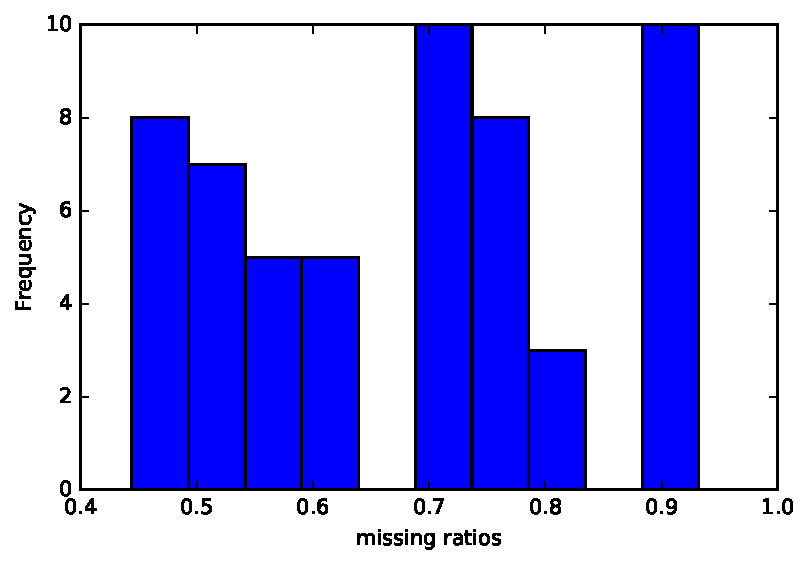
\includegraphics[width=0.6\textwidth]{missingRatio.pdf}
\caption{\label{fig:m1}The distribution of the ratio of missing values}
\end{figure}
%\begin{figure}
%\centering
%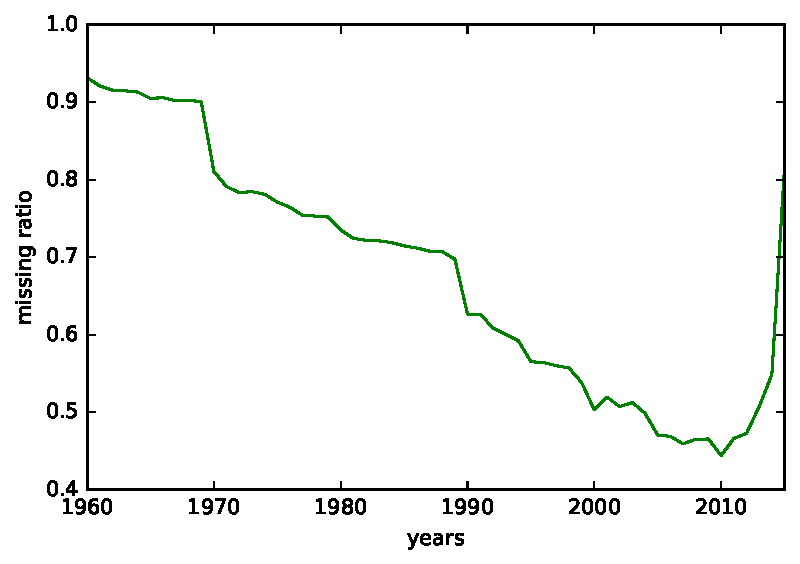
\includegraphics[width=0.8\textwidth]{missingByYear.pdf}
%\caption{\label{fig:m2}The trend of missing values by year}
%\end{figure}

It is observed that the missing ratio ranges from 0.4 to over 0.9, which justifies the high messiness of the dataset. As the missing ratio is lowest in Year 2010, the data from this year is extracted for our initial analysis.

It is also beneficial to understand  the correlation between these different indicators. Therefore,  Figure \ref{fig:c1} categorizes all the indicators into ten groups. 
\begin{figure}
\centering
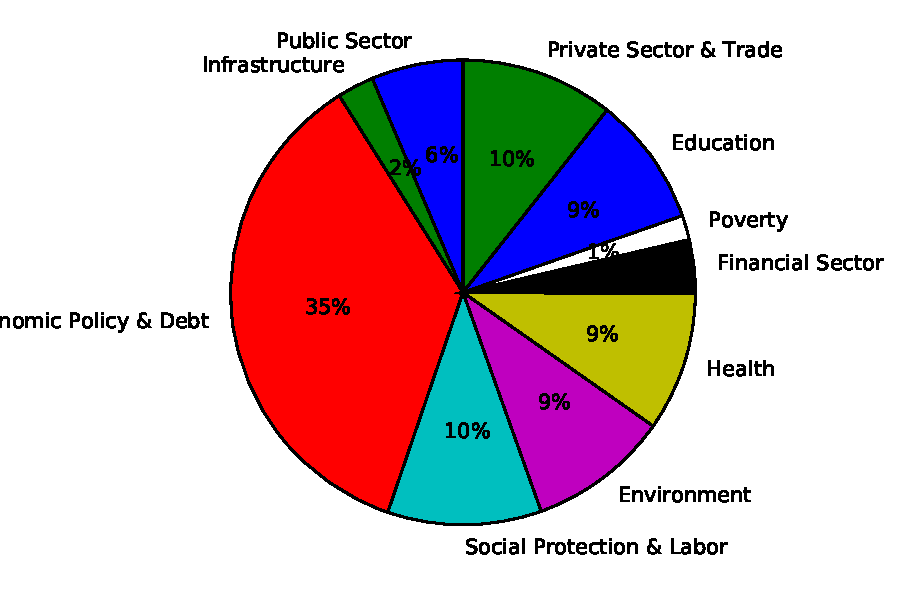
\includegraphics[width=0.6\textwidth]{category.pdf}
\caption{\label{fig:c1}Ten categories of all the indicators}
\end{figure}

From the pie chart, it is clear that majority of the indicators collected  belong to the economic policy and debt category, whereas the other indicators almost spread evenly onto the rest nine categories. It can also be further inferred that although the number of indicators is large, they are highly inter-correlated, which motivates the idea of feature selection. Therefore, in the later study, feature selection and clustering is implemented in each of the ten categories.
\subsection{Feature Selection and Extraction}
The combination of the high dimensionality, correlated features, and large amounts of missing data make feature selection, dimensionality reduction, and imputation methods critical to use before applying learning algorithms on this dataset.
Low-rank models provide ways to conduct all of these feature engineering steps on imperfect datasets. This is because they factor a large, possibly sparse dataset into dense, low-rank "thin" and "fat" factors that multiply to an approximation of the original dataset. Also, the loss function that is evaluated on the original dataset and its low-rank approximation can be evaluated only on observed entries, allowing a reconstruction to approximate missing values. This imputation allows partially-missing rows to be used in analysis instead of throwing away valuable data. In this low-rank approximation, the "thin" matrix represents transformed features while the "fat" matrix represents their transformations. We plan to use the LowRankModels.jl package to conduct this low-rank factorization.
\subsubsection{Reshaping}
The first item of preprocessing we had to do was a reshape operation so that a country-year pair was an observation and the indicators were features. This made the data more amenable to matrix-based learning algorithms such as low-rank models or linear regression. This transformation also reshaped our data from about 300,000 x 60 to about 15,000 x 1400.

\subsubsection{Removing Missing Columns}
Out of 1440 indicators, 109 were completely empty for every country, and several more were empty except for a low percentage (approximately 10\%) of the total number of rows. We removed these completely empty columns because imputation methods have no information on which to act for these columns. This left us with 1331 columns in our dataset.

\subsection{Intended Analyses}
After dimensionality reduction and imputation, we intend to develop classifications for the the different general topics, indicated by the first two characters of the column name. Since the classifications are ordinal variables, we intend to use ordinal clustering methods to determine where the levels lie. We will also develop the clusters for all features combined to determine how these cluster assignments change based on which features are included.
\section{Validation}
The unsupervised nature of our proposed analysis makes testing more difficult than in the supervised case. We intend to start by applying an ordinal clustering method to the economic indicators and comparing the results to the World Bank's published classifications, tuning our model by adjusting our dimensionality reduction approach and our clustering algorithm's tuning parameters. We will also fit an ordinal regression model for comparison to determine how much noise there may be in the data and how easy it is to obtain proper classifications.
\section{Future steps}
Our next steps involve further preprocessing to remove the columns and rows with too much missing data (fewer than 100 observations) so that imputation methods can have a chance of functioning. We will then fit dimensionality reduction algorithms such as robust PCA and quadratically regularized PCA to impute missing values and ease the fitting of clustering methods. Finally, we will conduct ordinal clustering on the economic topic of the dataset and tune the results to match the World Bank's classifications. After this, we would like to fit the same ordinal clustering method on the other topics to develop similar metrics for health, research, the environment, and other topics, as well as to draw insights on how the classifications and rankings of regions may vary on different indicators.
\end{document}